Our next example is especially weird.

\begin{prop}[Antipodal Sphere]
Let \(S = \{ (x,y,z) \in \RR^3 \mid x^2 + y^2 + z^2 = 1 \}\), and consider the equivalence relation \(\sigma\) on \(S\) such that \(x \,\sigma\, y\) if and only if \(y = \pm x\).
We define the set \(\mathbb{A} = S/\sigma\), and call the elements of \(\mathbb{A}\) \emph{antipodal pairs}.
We define a ternary relation on \(\mathbb{A}\) by \(\COLLINEAR{A}{B}{C}\) if and only if \[ \DET \begin{bmatrix} a_x & a_y & a_z \\ b_x & b_y & b_z \\ c_x & c_y & c_z \end{bmatrix} = 0. \] This relation is well-defined, and makes \(\mathbb{A}\) an incidence geometry which we call the \emph{antipodal sphere}.
\end{prop}

Before we approach this proof, notice that the ``points'' in this model are actually \emph{pairs} of ``points'' in \(\RR^3\).
Specifically, each point in \(\mathbb{A}\) is a set of the form \( \{ (\alpha, \beta, \gamma), (-\alpha, -\beta, -\gamma) \} \) for some real numbers \(\alpha, \beta, \gamma\) with \(\alpha^2 + \beta^2 + \gamma^2 = 1\).
Such pairs of points are called \emph{antipodes}.
We can think of these ``points'' as the intersection of the unit sphere with a line through the origin; see \autoref{fig:antipodal-sphere-point} for a picture.

\begin{figure}[h]
\begin{center}
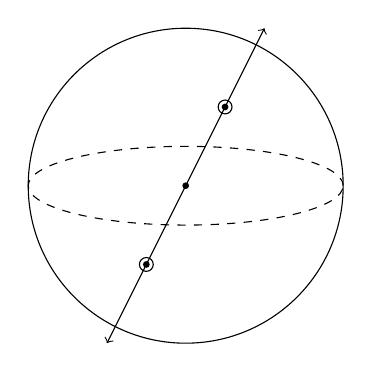
\begin{tikzpicture}[scale=0.5]
  \draw (0,0) circle (4);
  \draw [dashed] (0,0) ellipse (4 and 1);
  \draw [fill] (0,0) circle [radius=2pt];
  \draw [fill] (1,2) circle [radius=2pt];
  \draw [fill] (-1,-2) circle [radius=2pt];
  \draw (1,2) circle [radius=5pt];
  \draw (-1,-2) circle [radius=5pt];
  \draw [<->] (2,4) -- (-2,-4);
\end{tikzpicture}
\caption{\label{fig:antipodal-sphere-point}A ``point'' in the antipodal sphere (circled).}
\end{center}
\end{figure}
